\documentclass[oneside,final,14pt,a4paper]{extreport}

\usepackage{tempora}   

\usepackage{vmargin}
\setpapersize{A4}
\setmarginsrb{2.5cm}{2.2cm}{2.2cm}{2.2cm}{0pt}{10mm}{0pt}{13mm}
\usepackage{setspace}
\sloppy
\setstretch{1.5}
\usepackage{indentfirst}
\parindent=1.25cm

%%%%% ADDED TO SUPPORT TT BOLD FACES %%%%
\DeclareFontShape{OT1}{cmtt}{bx}{n}{<5><6><7><8><9><10><10.95><12><14.4><17.28><20.74><24.88>cmttb10}{}
\renewcommand{\ttdefault}{pcr}
%%%%% END %%%%%%%%%%%%%%%%%%%%%%%%%%%%%%% 
\usepackage{atbegshi,picture}
\usepackage[T1,T2A]{fontenc} 
\usepackage[utf8]{inputenc}
\usepackage[main=russian,english]{babel}
\usepackage[backend=biber,style=ieee,autocite=inline]{biblatex}
\bibliography{ref.bib}
\usepackage{csquotes}
\usepackage{blindtext}


\usepackage{pdfpages}
\newenvironment{bottompar}{\par\vspace*{\fill}}{\clearpage}

% \usepackage{cite}
\usepackage{amsmath,amsfonts}
\usepackage{amsthm}
\newtheorem{theorem}{Theorem}
\newtheorem{corollary}{Corollary}
\newtheorem{lemma}{Lemma}
\newtheorem{proposition}{Proposition}
\theoremstyle{definition}
\newtheorem{definition}{Definition}
\theoremstyle{remark}
\newtheorem*{remark}{Remark}
\theoremstyle{remark}
\newtheorem*{example}{Example}



\usepackage{graphicx}
\graphicspath{{figs/}} %path to images
\usepackage{multirow,array}
\usepackage{caption}
\usepackage{subcaption}
\usepackage[unicode]{hyperref}
\hypersetup{colorlinks=true, linkcolor=black, citecolor=black}
\usepackage{paralist}
\usepackage{listings}
\usepackage{zed-csp}
\usepackage{fancyhdr}
\usepackage{color,colortbl}
\usepackage{booktabs}
\usepackage{epsfig} % for postscript graphics files

\usepackage{upgreek} 
\usepackage{bm}
\usepackage{hyperref}
\usepackage{longtable}
\usepackage[font=singlespacing, labelfont=bf]{caption}
\usepackage{floatrow}

\pagestyle{fancyplain}

% remember section title
\renewcommand{\chaptermark}[1]%
	{\markboth{\chaptername~\thechapter~--~#1}{}}

% subsection number and title
\renewcommand{\sectionmark}[1]%
	{\markright{\thesection\ #1}}

\rhead[\fancyplain{}{\bf\leftmark}]%
      {\fancyplain{}{\bf\thepage}}
\lhead[\fancyplain{}{\bf\thepage}]%
      {\fancyplain{}{\bf\rightmark}}
\cfoot{} %bfseries


\newcommand{\dedication}[1]
   {\thispagestyle{empty}
     
   \begin{flushleft}\raggedleft #1\end{flushleft}
}

\begin{document}


\includepdf[offset=2.5cm -2.2cm]{title.pdf}

\newpage
\tableofcontents
\begin{abstract}
% skip one line to make the abstract start with indent

Моя аннотация начинается здесь.
\end{abstract}
\setcounter{page}{4}
% set manually the number, from which Глава 1 starts!
% Why do we put 4 in this case?
% Title page - page 1
% Оглавление - page 2
% Аннотация - page 3
% Глава 1 - page 4
% In your annotation the counter number can be different, please count carefully and insert the corresponding number.

\chapter{Introduction}
\label{chap:intro}
\chaptermark{Optional running chapter heading}
\section{Spacing \& Type}
\label{sec:section}

This is a section. This is a citation without brackets. and this is one with brackets \cite{A}. Multiple \cite{A,B,C} Here's a reference to a subsection: \ref{sec:subsection}. Citation of an online article \cite{D}. Citation of an online proceeding \cite{F}. The body of the text and abstract must be double-spaced except for footnotes or long quotations. Fonts such as Times Roman, Bookman, New Century Schoolbook, Garamond, Palatine, and Courier are acceptable and commonly found on most computers. The same type must be used throughout the body of the text. The font size must be 10 point or larger and footnotes\footnote{This is a footnote.} must be two sizes smaller than the text\footnote{This is another footnote.} but no smaller than eight points. Chapter, section, or other headings should be of a consistent font and size throughout the ETD, as should labels for illustrations, charts, and figures.

\subsection{Creating a Subsection}
\label{sec:subsection}

\subsubsection{Creating a Subsubsection}
\subsubsection{Creating a Subsubsection}
\subsubsection{Creating a Subsubsection}

\paragraph{This is a heading level below subsubsection}

And this is a quote: 
%
\begin{quote}
\blindtext
\end{quote}

\begin{figure}[hbt]
\centering

\includegraphics[]{figs/images.png}
\caption{One kernel at $x_s$ (\emph{dotted kernel}) or two kernels at
$x_i$ and $x_j$ (\textit{left and right}) lead to the same summed estimate
at $x_s$. This shows a figure consisting of different types of
lines. Elements of the figure described in the caption should be set in
italics, in parentheses, as shown in this sample caption.}
\label{fig:example}
\end{figure}

This is a table:
% currsize is not set in the long table environment, so we need to set it before we set it up.
\makeatletter
\let\@currsize\normalsize
\makeatother

% tabular environments are set to be single-spaced in the  thesis class,  but long tables do not use tabular
% to get around this, set the spacing to single spacing at the start of the long table environment, and set it back to double-spacing at the end of it

\begin{longtable}{c|c|c}
\caption[This is the title I want to appear in the List of Tables]{This Is a Table Example} \label{tab:pfams} \\
\hline
A & B & C \\
\hline
\endfirsthead
\multicolumn{3}{@{}l}{} \\
\hline
A & B & C\\
\hline
\endhead
a1 & b1 & c1 \\
a2 & b2 & c2\\
a3 & b3 & c3\\
a4 & b4 & c4\\
\hline
\end{longtable}

The package ``upgreek'' allows us to use non-italicized lower-case greek letters. See for yourself: $\upbeta$, $\bm\upbeta$, $\beta$, $\bm\beta$. Next is a numbered equation:
\begin{align}
\label{eq:name}
\|\bm{X}\|_{2,1}={\underbrace{\sum_{j=1}^nf_j(\bm{X})}_{\text{convex}}}=\sum_{j=1}^n\|\bm{X}_{.,j}\|_2
\end{align}
The reference to equation (\ref{eq:name}) is clickable. 
\section[Theorems, Corollaries, Lemmas, Proofs, Remarks, Definitions and Examples]{Theorems, Corollaries, Lemmas, Proofs, Remarks, Definitions,and Examples}

\begin{theorem}
\label{thm:onlytheorem}
\blindtext
\end{theorem}

\begin{proof}
I'm a (very short) proof.
\end{proof}

\begin{lemma}
I'm a lemma.
\end{lemma}

\begin{corollary}
I include a reference to Thm. \ref{thm:onlytheorem}.
\end{corollary}

\begin{proposition}
I'm a proposition.
\end{proposition}

\begin{remark}
I'm a remark. 
\end{remark}

\begin{definition}
I'm a definition. I'm a definition. I'm a definition. I'm a definition. I'm a definition. I'm a definition. I'm a definition. I'm a definition. I'm a definition. I'm a definition. I'm a definition. 
\end{definition}

\begin{example}
I'm an example.
\end{example}


\section[Optional table of contents heading]{Section with\\ linebreaks in\\the
name}


\Blindtext[2]





\chapter{Обзор литературы}
\label{chap:background}

\chapter{Processor Scheduling Strategies}
\label{chap:processorSchedulingStrategies}
We provide the necessary preliminaries for our heterogeneous scheduling analysis. We start with a homogeneous scheduling case with identical processors in Section~\ref{sec:singleProcessor} and~\ref{sec:homogeneousMultiprocessorCase}. Then, we describe the basic heterogeneous scheduling principles in Section~\ref{sec:heterogeneousCase}. We especially focus on various scheduling overheads in regard to these principles in Section~\ref{sec:performanceOverheads}.


\section{Single processor case}
\label{sec:singleProcessor}

\begin{figure*}
\begin{minipage}{.75\columnwidth}%
\begin{subfigure}[t]{\linewidth}
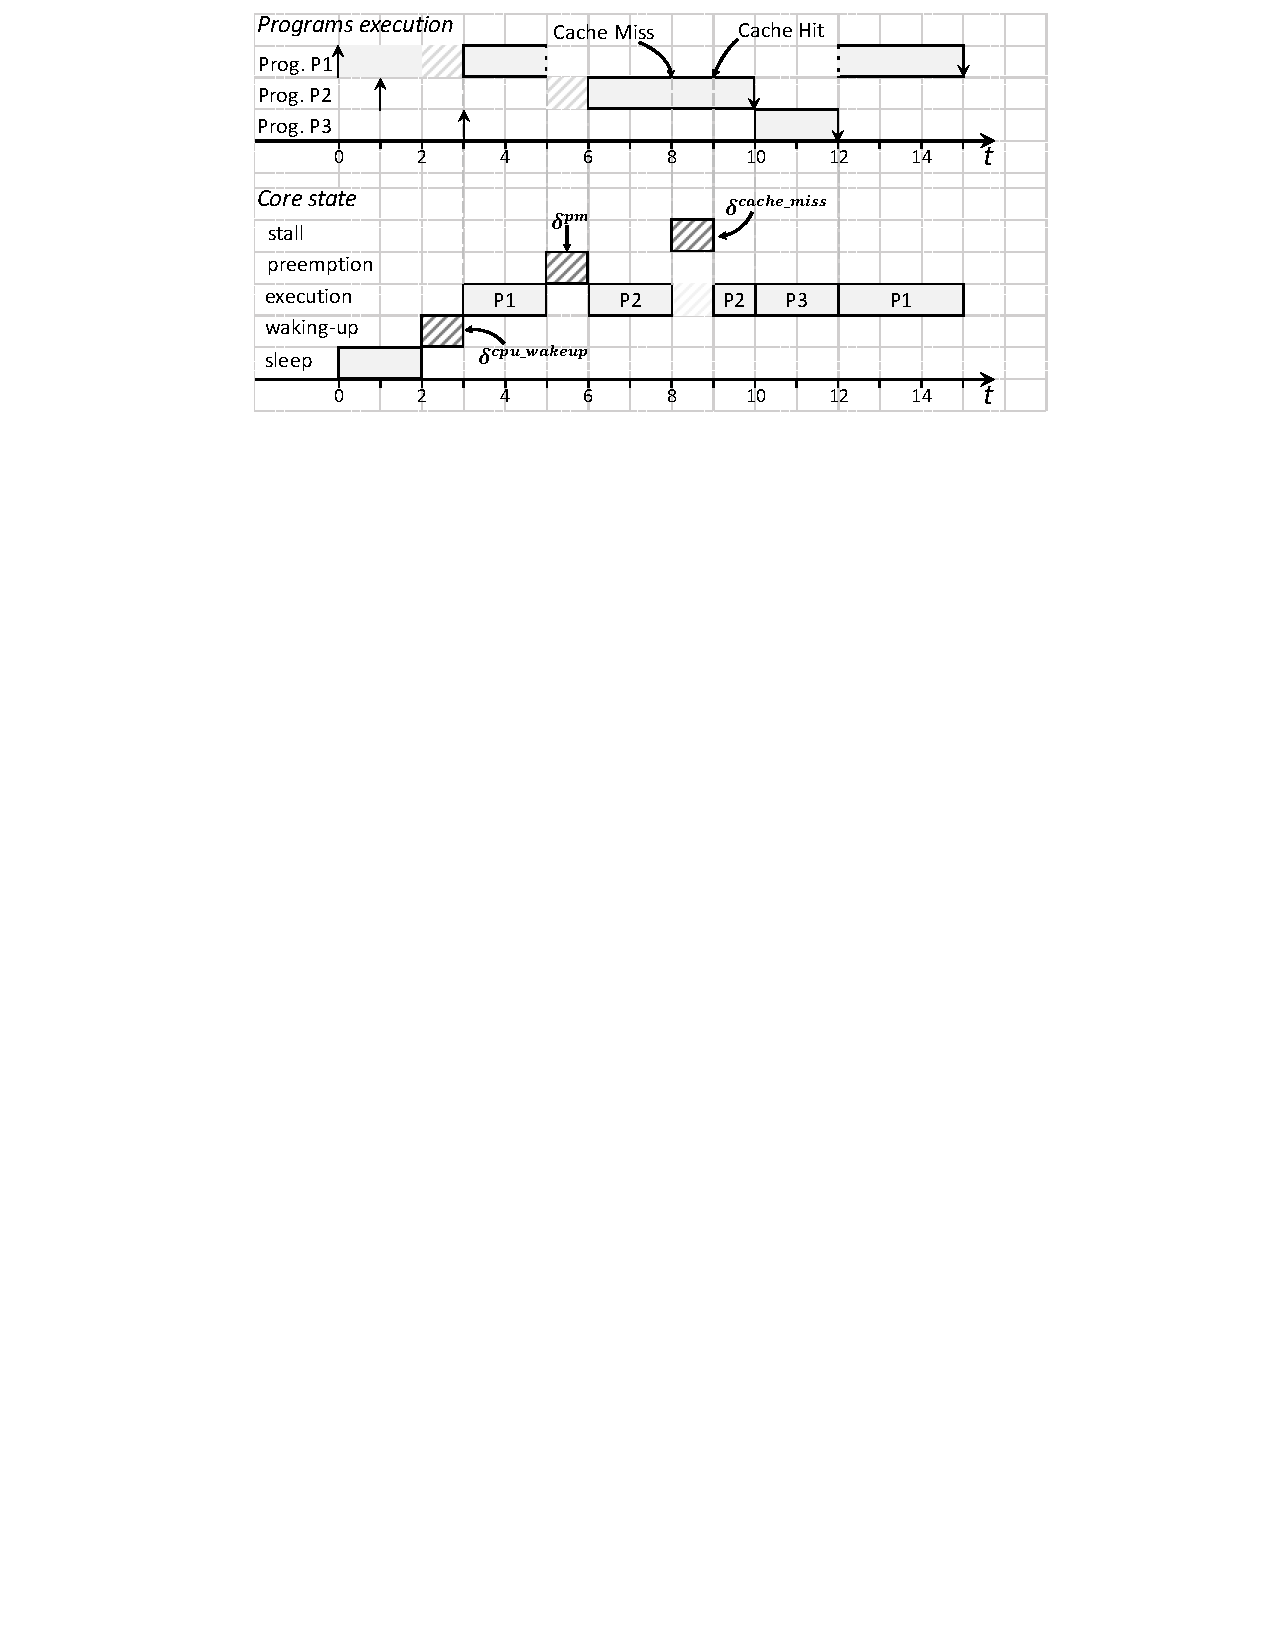
\includegraphics[width=\linewidth]{figs/singleProcessorExecutionExample.pdf}
\caption{Single processor executing three programs with requirements in Fig.~\ref{fig:singleProcessorExampleRequirements}.}
\vspace{3mm}
\label{fig:singleProcessorExecutionExample}
\end{subfigure}
\begin{subfigure}[t]{\linewidth}
%\hspace{21.5mm}
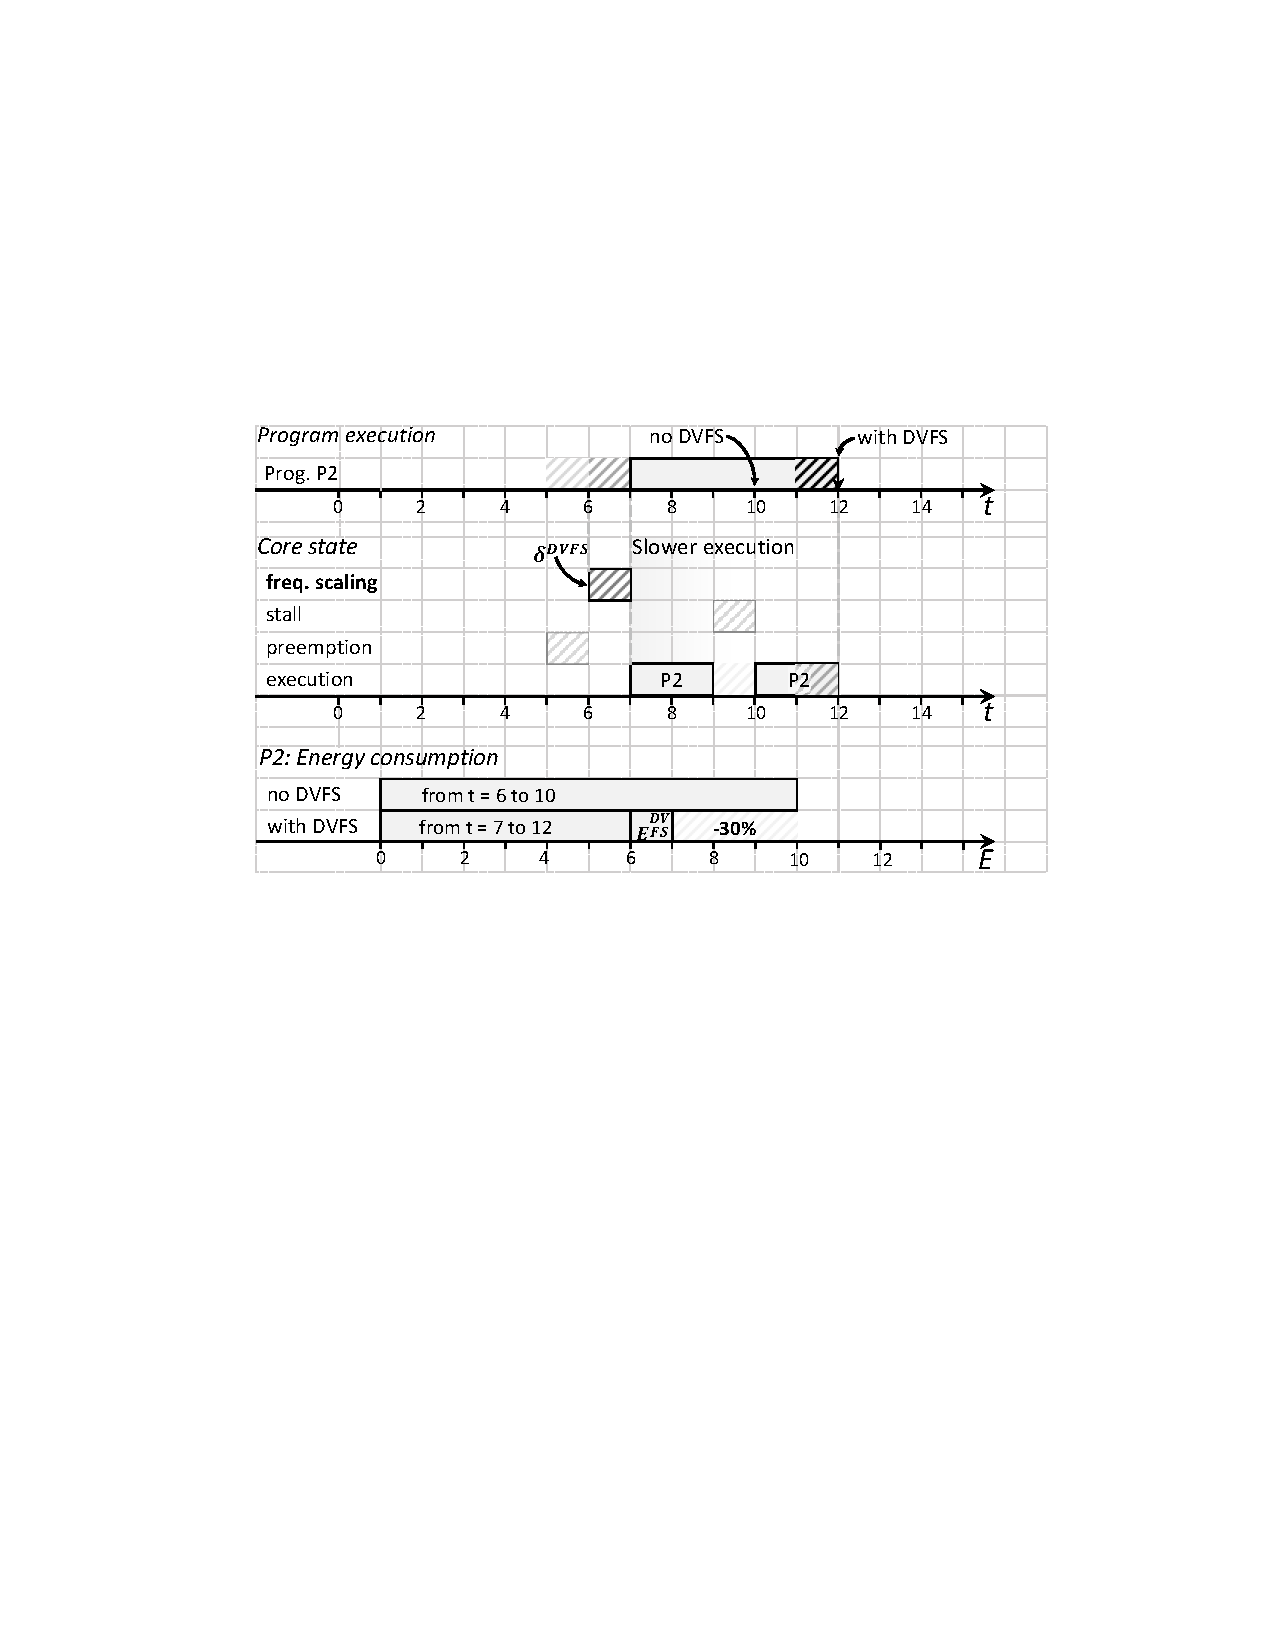
\includegraphics[width=\linewidth]{figs/DVFSExample.pdf}
\caption{Program $P_2$ execution with DVFS enabled}
\vspace{3mm}
\label{fig:DVFSExample}
\end{subfigure}
\begin{subfigure}[t]{\linewidth}
%\vspace{-65mm}
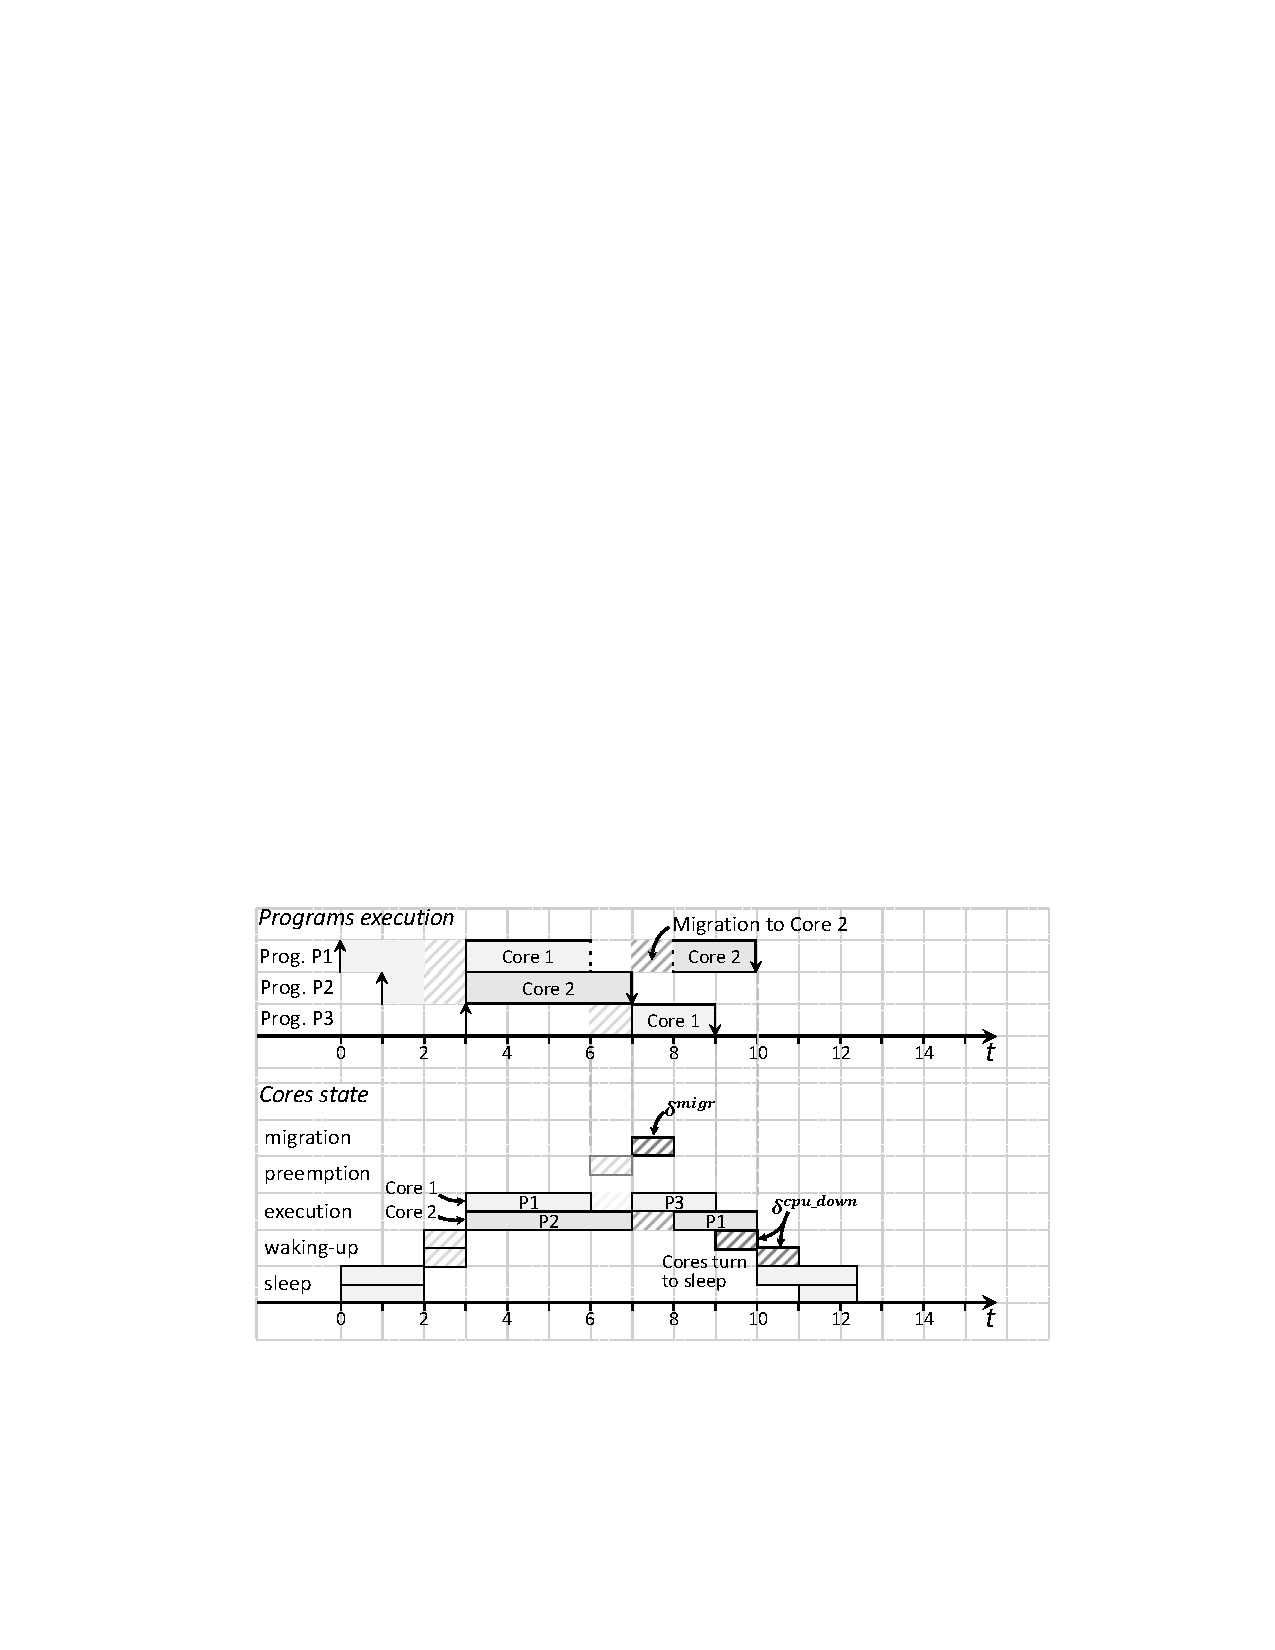
\includegraphics[width=\linewidth]{figs/multiprocessorExecutionExample.pdf}
\caption{Programs execution over 2 ``no DVFS" cores with requirements in Fig.~\ref{fig:singleProcessorExampleRequirements}}
\vspace{3mm}
\label{fig:multiprocessorExecutionExample}
\end{subfigure}
\end{minipage}

\caption{Single and multi-processor programs execution}
\label{fig:singleProcessorCase}
\quad
\end{figure*}

\begin{figure}
\centering
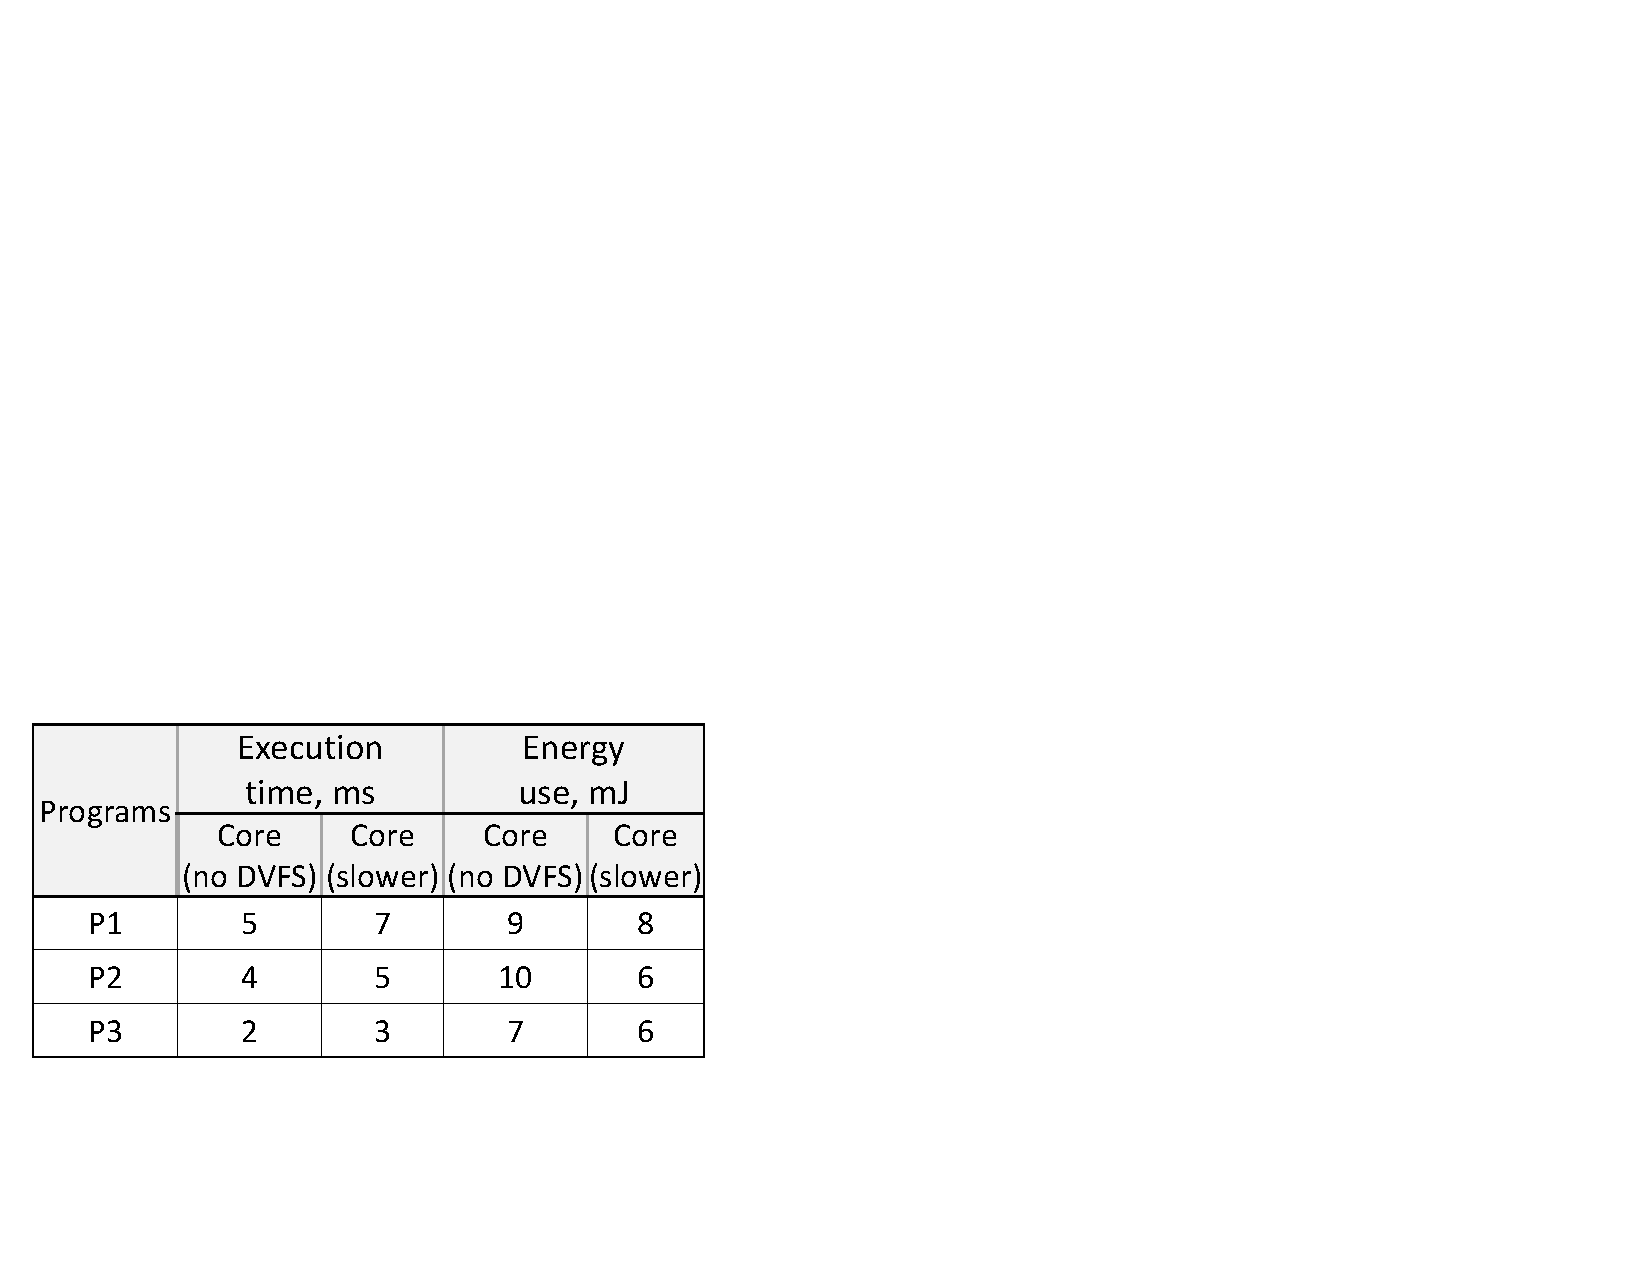
\includegraphics[width=.65\linewidth]{figs/singleProcessorExampleRequirements.pdf}
\caption{Programs requirements for a single core}
\label{fig:singleProcessorExampleRequirements}
\end{figure}


%\begin{figure}
%\centering
%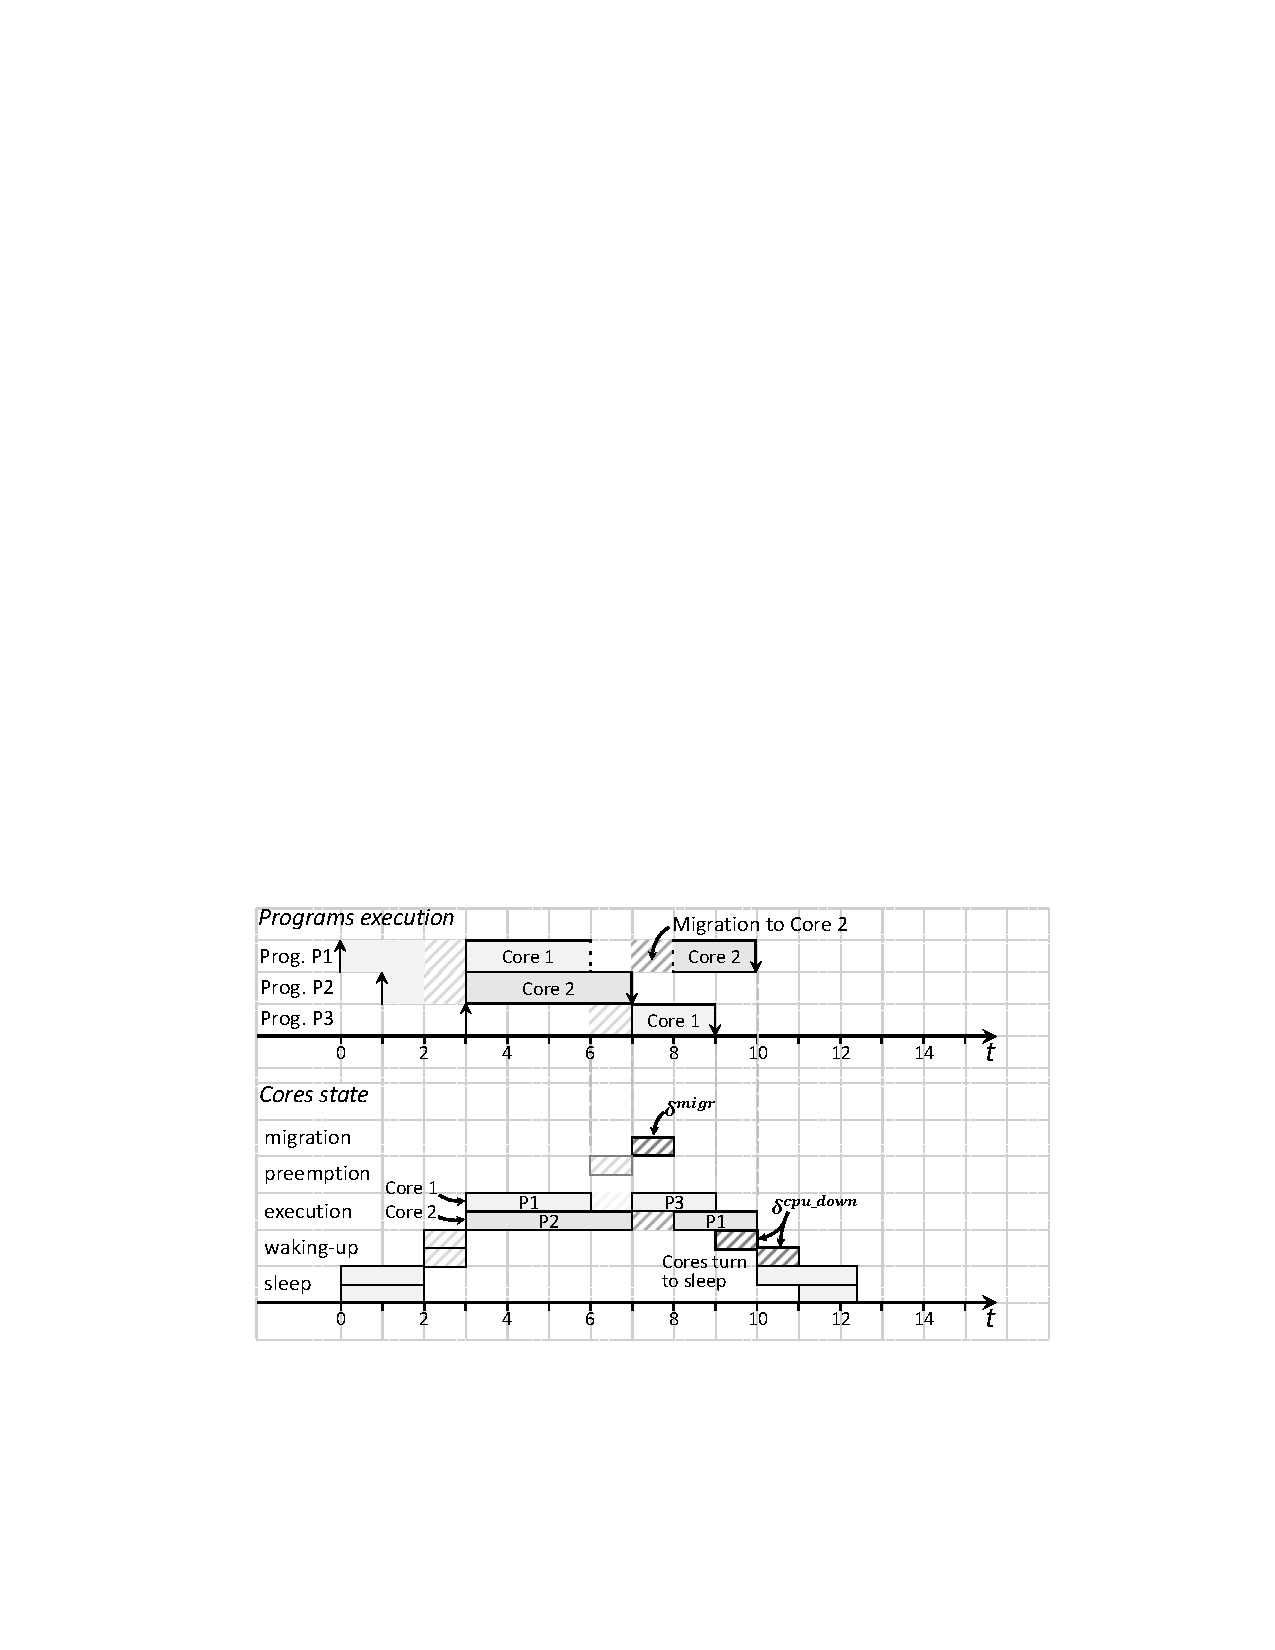
\includegraphics[width=\columnwidth]{figs/multiprocessorExecutionExample.pdf}
%\caption{Programs execution over 2 ``fast" cores with requirements in Fig.~\ref{fig:singleProcessorExampleRequirements}}
%\label{fig:multiprocessorExecutionExample}
%\end{figure}

Consider an execution schedule of Fig.~\ref{fig:singleProcessorExecutionExample}. Three programs labeled P1, P2 and P3 execute over a same shared single core. Programs execution requirements are listed in Fig.~\ref{fig:singleProcessorExampleRequirements}. The scenario of Fig.~\ref{fig:singleProcessorExecutionExample} assumes programs P1, P2 and P3 to arrive at times $t=0$, $1$ and $3$ correspondingly.

Observe that in the presented execution schedule more than 30\% of its duration is wasted on core overheads due to its transitions between execution and other states. In fact, this is a highly relevant problem for realistic systems, so that it must be carefully accounted when making scheduling decisions.

%Let us focus on the most interesting aspects of this schedule. Observe that programs await for execution for quite a significant time due to the core performance overheads, including core transitions between operational modes and preemptions (66\% of the schedule duration)

%\begin{enumerate}
%\itemindent=18pt
%\item[$t=0$:] P1 arrives, while a core is in a sleep mode;
%\item[$t=1$:] P2 arrives, but the core is not yet waken up;
%\item[$t=2$:] P1 and P2 do not yet execute, but the core wakens;
%\item[$t=3$:] P1 executes as the core is awake, while P3 arrives;
%\item[$t=5$:] P1 is preempted by P2 due to a scheduling policy\footnote{The discussion of various scheduling prioritization policies is later in Section X};
%\item[$t=8$:] P2 is blocked as the core stalls on a cache miss;
%\itemindent=23pt
%\item[$t=10$:] P2 completes, P3 executes and P1 is pending;
%\end{enumerate}

%Note that sleep/awake core states transition, programs preemption and cache misses impose significant additional overheads. 

Modern cores actually support a varying execution speed due to so-called Dynamic Voltage and Frequency Scaling (DVFS). However, DVFS again imposes additional performance overheads. As an illustration, consider an execution in Fig.~\ref{fig:DVFSExample}, assuming programs requirements for a slower core are listed in Fig.~\ref{fig:singleProcessorExampleRequirements}. Starting from $t=6$, the execution is as following:
\begin{enumerate}
\itemindent=18pt
\item[$t=6$:] Core's frequency decreases;
\item[$t=7$:] P2 executes;
\item[$t=9$:] The core stalls (see Fig.~\ref{fig:singleProcessorExecutionExample});
\itemindent=23pt
\item[$t=12$:] P2 completes;
\end{enumerate}

Below we summarize energy consumed for P2 execution. Note that use of DVFS significantly reduced it from 10 to 6 units at moderate performance degradation.



\section{Homogeneous multiprocessor case}
\label{sec:homogeneousMultiprocessorCase}

A sample multiprocessor execution~\cite{Gepner2006,Chai2007,Kumar2003, Nayfeh1997, Geer2005} is provided in  Fig.~\ref{fig:multiprocessorExecutionExample}, assuming cores are homogeneous that is they provide same execution speed without DVFS. The figure illustrates the following:
\begin{enumerate}
\itemindent=18pt
\item[$t=0$:] P1 arrives, both cores sleep;
\item[$t=1$:] P2 arrives;
\item[$t=2$:] Cores wake up;
\item[$t=3$:] P1 starts on Core 1, P2 \-- on Core 2, P3 arrives;
\item[$t=6$:] P3 preempts P1 on Core 1;
\item[$t=7$:] P2 completes, P1 migrates to Core 2;
\item[$t=9$:] P3 completes, Core 1 turns down;
\itemindent=23pt
\item[$t=10$:] P1 completes, Core 2 turns down;
\end{enumerate}

Compared to a single processor case, the programs are completed at time 10 instead of 15. Also, a multiprocessor allowed programs to migrate between cores and to execute in a single core mode (from $t=9$ in Fig.~\ref{fig:multiprocessorExecutionExample}) by turning down cores. Although, both migrations and awake/sleep transitions impose additional time overheads.


\section{Heterogeneous multiprocessor case}
\label{sec:heterogeneousCase}

Heterogeneous hardware (HW) contains processing units of different types, such as CPU, GPU, TPU and NPU~\cite{Brodtkorb2010}. Some of them are designed for general-purpose computational tasks, such as single- or multicore Central Processing Units (CPU) used for operating systems management, while others \-- for application-specific tasks, such as Graphic, Tensor or Neural Processing Units (GPU, TPU, NPU) used for Artificial Intelligence training and inference tasks.

Despite significant variation in execution speed and energy consumption, these PUs share common HW organizational principles originally coming from a classical single processor case described in Section~\ref{sec:singleProcessor}. In fact, the major key differences are in the number of cores and supported instruction sets. For example, in Fig.~\ref{fig:bigLITTLEArchitecture} the ``big" cluster provides only four cores, while GPU and NPU provide thousands and hundreds respectively.

\begin{figure*}
\begin{minipage}{.75\columnwidth}%
\begin{subfigure}{1.105\linewidth}
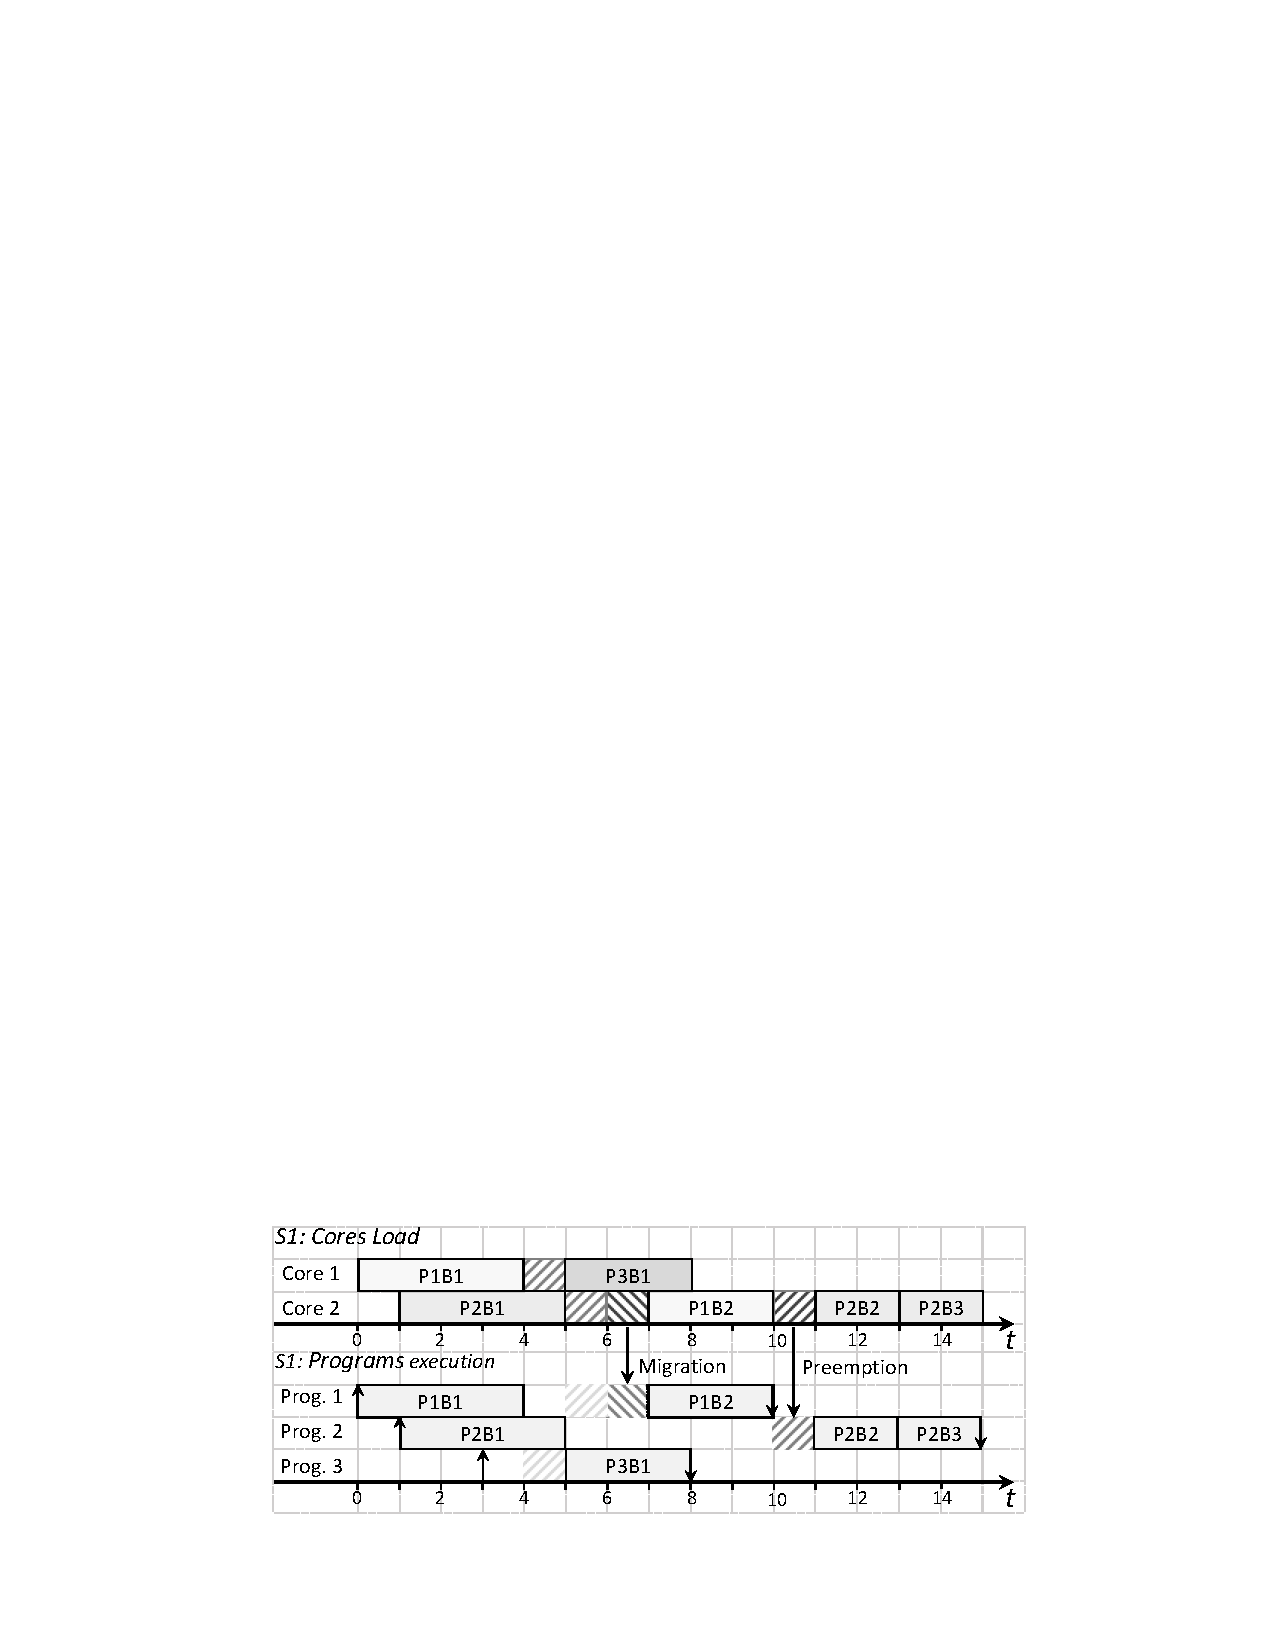
\includegraphics[width=\linewidth]{figs/s1PreemptionMigration.pdf}
%\vspace{3mm}
\end{subfigure}
\caption{Schedule S1 with preemptions and migrations considered}
\label{fig:s1PreemptionMigration}
\end{minipage}%
\quad
\end{figure*}


\subsection*{\textbf{Common execution principles}}

We illustrate a concurrent programs execution upon different PU types, considering preemptions and migrations, in Fig.~\ref{fig:s1PreemptionMigration}, which extends the Schedule S1 of our toy example. The programs execute as following:
\begin{enumerate}
\itemindent=14pt
\item[$t=0$:] P1 starts on Core 1;
\item[$t=1$:] P2 starts on Core 2;
\item[$t=4$:] P3 preempts P1;
\item[$t=5$:] P1 preempts P2;
\item[$t=6$:] P1 migrates to Core 2;
\item[$t=7$:] P1 resumes.
\end{enumerate}

Both preemptions and migrations require a context switch, which is to save the state of a preempted program and load the preemptee's. Such a context switch impose significant performance overhead, which in reality vary from tens to hundreds microseconds \cite{Mogul1991, David2007, McVoy1996}.

%inquiring 0.2-1.7\% of utilization in an average case and up to 10\% in the worst case scenario \todo{put references to percentages}.


\section{Scheduling types and overheads}
\label{sec:heterogeneousScheduling}

In our toy example we assume preemptions and migrations are possible. In reality, this is not always a case. Next, we describe different schedules types as well as summarize time overheads relevant for our analysis.
%We relax this assumption in Fig.~\ref{fig:executionWithPreemptionMigration} extending the Schedule S1 to consider preemptions and migrations overheads. For simplicity, we assume both preemptions and migrations require 1 time unit. 

\subsection*{\textbf{Scheduling types}}
\label{sec:schedulingTypes}

We distinguish scheduling types from the preemptiveness and migrativeness perspectives. A program execution is:
%
\begin{itemize}
\item{Preemptive:} it can be preempted by another program;
\item{Non-preemptive:} once started, it cannot be preempted;
\item{Migrative:} it can migrate between processing units (PUs);
\item{Non-migrative:} it is statically assigned to a specific PU.
\end{itemize}

A preemption might occur either at any time or at a completion time of a program block\footnote{The definition of a program block is to be elaborated later}. For example, in Fig.~\ref{fig:s1PreemptionMigration} preemptions occur at $t=4$ and $5$ after completion of the first blocks of Prog. P1 and P2 correspondingly, while migration \-- at $t=6$ when P1 switched from Core 1 to Core 2.

We note that execution preemptions and migrations on one side provide scheduling flexibility\footnote{The flexibility in programs prioritization policy, different scheduling types and other improves hardware utilization}, but however at additional overhead costs. As an example, consider the execution schedule in Fig.~\ref{fig:s1PreemptionMigration}: Core 2 spends 11 time units for programs execution and 3 for context switches, which is 20\% of its operational time. Anyway, both preemptions and migrations are widely used and incomparable from the performance perspective. Preemptions offer increased processor utilization, while migrations \-- reduced programs execution time. For example, in Fig.~\ref{fig:twoSchedulesExample} Schedule S2 has no migrations and greater total execution time comparing to S1, which has 1 migration. 

%\todo{AB@AM: To rethink either we should limit our analysis scope to a specific scheduling type.} In our analysis we assume the block-level preemptive and migrative scheduling.

\subsection*{\textbf{Performance overheads}}
\label{sec:performanceOverheads}

Any scheduler imposes various hardware-related execution overheads, which are related to principles discussed in Chapter.~\ref{chap:processorSchedulingStrategies}, such as preemptiveness and migrativeness, cache misses, and other:

\begin{itemize}
\item Preemptive and migrative programs execution:
%
\begin{itemize}
\itemindent=8pt
\item[$\delta^{\mathsf{pm}}$\--] preemption overhead;
\itemindent=12pt
\item[$\delta^{\mathsf{migr}}$\--] migration overhead.
\end{itemize}

\item Processing unit mode:
%
\begin{itemize}
\itemindent=37pt
\item[$\delta^\mathsf{{cpu\_wakeup}}$\--] time overhead related to an operational mode switch;
\itemindent=31	pt
\item[$\delta^\mathsf{{cpu\_down}}$\--] time overhead related to a sleep mode switch.
\end{itemize}

\item Dynamic Voltage and Frequency Scaling (DVFS):
%
\begin{itemize}
\itemindent=18pt
\item[$\delta^\mathsf{{DVFS}}$\--] time overhead related to the processing frequency adjustment.
\end{itemize}

\item Cache hits and misses:
%
\begin{itemize}
\itemindent=40pt
\item[$\delta^\mathsf{{cache\_miss}}$ \--] time overhead related to a cache miss.
\end{itemize}
\end{itemize}

\section{Existing heterogeneous schedulers}
\label{sec:existingSchedulers}

Several heterogeneous schedulers are proposed in the literature, including 
Heterogeneous Earliest-Finish-Time (HEFT)~\cite{Topcuoglu1999, Topcuoglu2002, Bittencourt2010, Samadi2018},
Critical-Path-on-a-Processor (CPOP)~\cite{Topcuoglu2002, Topcuoglu1999}, 
StarPU~\cite{Augonnet2009}, 
Fast Load Balancing (FLP)~\cite{Radulescu1999, Radulescu2000}, 
Fast Critical Path (FCP)~\cite{Radulescu1999_FCP, Radulescu2000}, and 
Heterogeneity-Aware Signature-Supported scheduler (HASS)~\cite{Shelepov2009}. 
These schedulers are however provide suboptimal solutions based on different heuristics. Some of them employ fixed priority assignments for programs, although without any knowledge about the optimality of those priorities. Other schedulers use greedy time optimization, static cores allocations (also known as partitioned scheduling), and other.
\chapter{Implementation}
\label{chap:impl}

\ldots
\chapter{Выводы}
\label{chap:conclusion}


\printbibliography[heading=bibintoc,title={Список использованной литературы}]
\end{document}

